% ============================================================
% Reporte: Conversión de Minúsculas a Mayúsculas en Ensamblador x86
% Autor: Edson Joel Carrera Avila
% ============================================================

\documentclass[12pt, letterpaper]{article}

\usepackage[utf8]{inputenc}
\usepackage[T1]{fontenc}
\usepackage[english]{babel}
\usepackage{geometry}
\usepackage{graphicx}
\usepackage{listings}
\usepackage{xcolor}
\usepackage{booktabs}
\usepackage{amsmath}
\usepackage{hyperref}
\usepackage{fancyhdr}
\usepackage{float}
\usepackage{caption}
\usepackage{tikz}
\usetikzlibrary{shapes.geometric, arrows.meta, positioning}

\geometry{top=2.5cm, bottom=2.5cm, left=3cm, right=2.5cm}

% --- Colores y estilo de código ---
\definecolor{codegray}{rgb}{0.95,0.95,0.95}
\definecolor{codegreen}{rgb}{0.0,0.5,0.0}
\definecolor{codeblue}{rgb}{0.0,0.0,0.65}
\definecolor{codepurple}{rgb}{0.45,0.0,0.55}

\lstdefinelanguage{MASM}{
    morekeywords={PROC,ENDP,END,PUSH,POP,MOV,ADD,SUB,CALL,RET,JMP,
                  JE,JB,JA,INC,CMP,EXTERN,BYTE,DWORD,QWORD,PTR,
                  EBP,ESP,ESI,AL,.586,.model,.data,.code,flat,stdcall,offset},
    sensitive=false,
    morecomment=[l]{;}
}

\lstset{
    backgroundcolor=\color{codegray},
    basicstyle=\ttfamily\footnotesize,
    keywordstyle=\color{codeblue}\bfseries,
    commentstyle=\color{codegreen}\itshape,
    numbers=left, numberstyle=\tiny\color{gray}, numbersep=8pt,
    frame=single, rulecolor=\color{gray!50},
    breaklines=true, captionpos=b, tabsize=4,
    showstringspaces=false,
    literate=
        {á}{{\'a}}1 {é}{{\'e}}1 {í}{{\'i}}1 {ó}{{\'o}}1 {ú}{{\'u}}1
        {Á}{{\'A}}1 {É}{{\'E}}1 {Í}{{\'I}}1 {Ó}{{\'O}}1 {Ú}{{\'U}}1
        {ñ}{{\~n}}1 {Ñ}{{\~N}}1
}

% --- Encabezado ---
\pagestyle{fancy}
\fancyhf{}
\rhead{Práctica 01 --- Conversión Minúsculas a Mayúsculas en ASM}
\lhead{\textit{Edson Joel Carrera Avila}}
\cfoot{\thepage}
\renewcommand{\headrulewidth}{0.5pt}

% ============================================================
\begin{document}

% --- Portada ---
\begin{titlepage}
    \centering
    \vspace*{1.5cm}

    {\Large \textbf{Universidad Autónoma de la Ciudad de México}}\\[0.3cm]
    {\large Licenciatura en Ingeniería de Software}\\[0.2cm]
    {\large Arquitectura de Computadoras}\\[2.5cm]

    \rule{\linewidth}{0.5pt}\\[0.4cm]
    {\LARGE \bfseries Práctica 01}\\[0.3cm]
    {\Large Conversión de Minúsculas a Mayúsculas en Ensamblador x86}\\[0.3cm]
    \rule{\linewidth}{0.5pt}\\[2cm]

    \begin{flushleft}
        \textbf{Alumno:} Edson Joel Carrera Avila \\[0.3cm]
        \textbf{Grupo:} 302 \\[0.3cm]
        \textbf{Profesor:} Prof. Mtro. Omar Nieto Crisóstomo \\[0.3cm]
        \textbf{Fecha:} \today
    \end{flushleft}
    \vfill
\end{titlepage}

\tableofcontents
\newpage

% ============================================================
\section{Introducción}

Esta práctica consiste en escribir un programa en \textbf{lenguaje ensamblador x86} que tome una cadena de texto y convierta todas sus letras minúsculas en mayúsculas, sin usar ninguna función externa: todo el trabajo lo hace el programa por sí solo, directamente sobre la memoria de la computadora.

El objetivo principal no es simplemente ``poner letras en mayúscula'', sino entender cómo una computadora representa y manipula texto a su nivel más básico. Para lograrlo, es necesario comprender dos conceptos fundamentales: la \textbf{tabla ASCII} y el \textbf{acceso directo a memoria}.

\subsection*{¿Qué es la tabla ASCII?}

Las computadoras no almacenan letras directamente; almacenan números. La tabla ASCII (por sus siglas en inglés: \textit{American Standard Code for Information Interchange}) es un acuerdo universal que asigna un número a cada carácter. Por ejemplo:

\begin{table}[H]
    \centering
    \begin{tabular}{@{}ccc@{}}
        \toprule
        \textbf{Carácter} & \textbf{Valor decimal} & \textbf{Tipo} \\
        \midrule
        \texttt{A} & 65  & Mayúscula \\
        \ldots      & \ldots & \ldots \\
        \texttt{Z} & 90  & Mayúscula \\
        \midrule
        \texttt{a} & 97  & Minúscula \\
        \ldots      & \ldots & \ldots \\
        \texttt{z} & 122 & Minúscula \\
        \bottomrule
    \end{tabular}
    \caption{Fragmento relevante de la tabla ASCII}
\end{table}

La observación clave es que \textbf{toda letra minúscula tiene un valor exactamente 32 unidades mayor que su correspondiente mayúscula}. Por lo tanto, para convertir de minúscula a mayúscula basta con \textbf{restar 32} al número que representa al carácter:

\begin{equation}
    \text{mayúscula} = \text{minúscula} - 32
\end{equation}

% ============================================================
\section{Organización del programa}

El proyecto consta de un único archivo:

\begin{table}[H]
    \centering
    \begin{tabular}{@{}lp{9cm}@{}}
        \toprule
        \textbf{Archivo} & \textbf{Qué hace} \\
        \midrule
        \texttt{conversion.asm} & Declara la cadena de texto en memoria, la recorre carácter por carácter y convierte las minúsculas a mayúsculas. \\
        \bottomrule
    \end{tabular}
    \caption{Archivo del proyecto}
\end{table}

El programa se divide internamente en dos secciones:

\begin{itemize}
    \item \textbf{Sección \texttt{.data}:} es donde se declara y almacena la cadena de texto inicial en la memoria del programa.
    \item \textbf{Sección \texttt{.code}:} contiene las instrucciones que el procesador ejecuta una por una para recorrer y modificar esa cadena.
\end{itemize}

El flujo general del programa es el siguiente:

\begin{figure}[H]
    \centering
    \resizebox{0.8\textwidth}{!}{%
        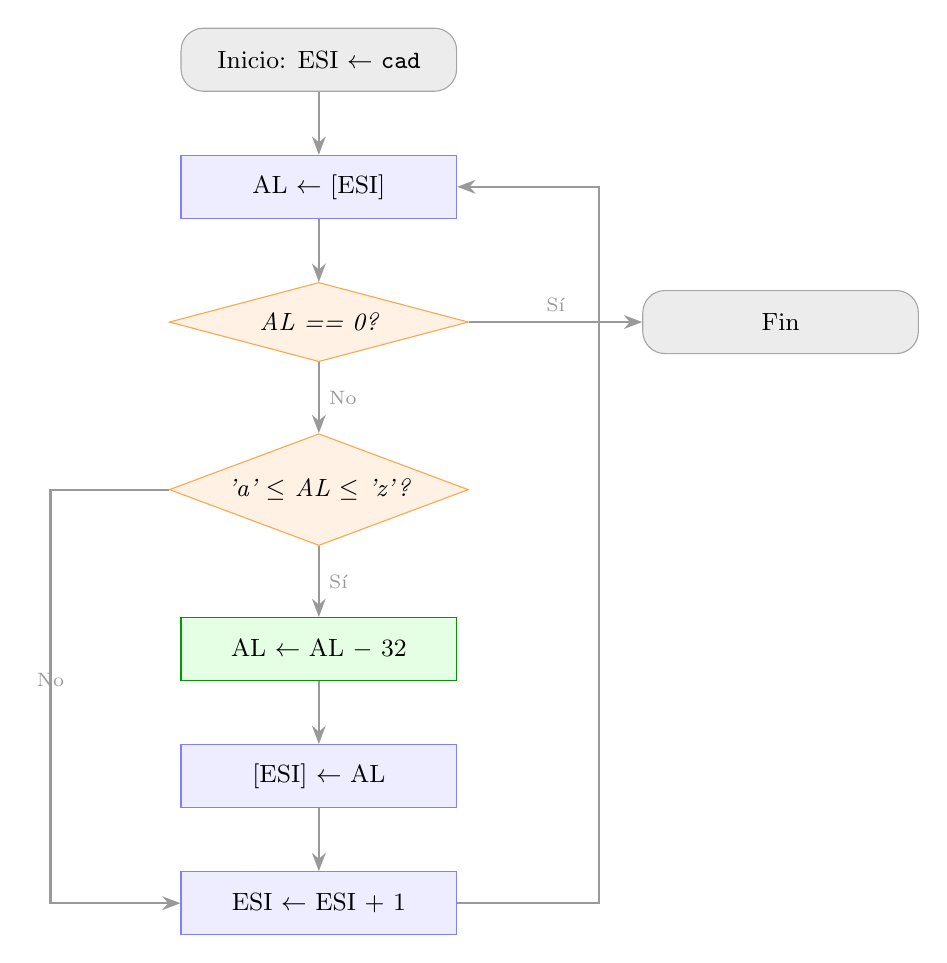
\begin{tikzpicture}[
            startstop/.style={rectangle, rounded corners=8pt, draw=gray!70, fill=gray!15,
                              minimum width=3.5cm, minimum height=0.8cm, font=\small},
            process/.style  ={rectangle, draw=blue!50, fill=blue!7,
                              minimum width=3.5cm, minimum height=0.8cm, font=\small},
            decision/.style ={diamond, aspect=2.2, draw=orange!70, fill=orange!10,
                              minimum width=3.8cm, font=\small\itshape, inner sep=1pt},
            convert/.style  ={rectangle, draw=green!60!black, fill=green!10,
                              minimum width=3.5cm, minimum height=0.8cm, font=\small},
            arr/.style      ={-Stealth, thick, gray!80}
        ]
            \node[startstop] (inicio)   {Inicio: ESI $\leftarrow$ \texttt{cad}};
            \node[process,   below=0.8cm of inicio]  (leer)    {AL $\leftarrow$ [ESI]};
            \node[decision,  below=0.8cm of leer]    (es0)     {AL == 0?};
            \node[startstop, right=2.2cm of es0]     (fin)     {Fin};
            \node[decision,  below=0.9cm of es0]     (rango)   {'a' $\leq$ AL $\leq$ 'z'?};
            \node[convert,   below=0.9cm of rango]   (conv)    {AL $\leftarrow$ AL $-$ 32};
            \node[process,   below=0.8cm of conv]    (escribe) {[ESI] $\leftarrow$ AL};
            \node[process,   below=0.8cm of escribe] (inc)     {ESI $\leftarrow$ ESI $+$ 1};

            \draw[arr] (inicio)  -- (leer);
            \draw[arr] (leer)    -- (es0);
            \draw[arr] (es0)     -- node[above, font=\scriptsize]{Sí} (fin);
            \draw[arr] (es0)     -- node[right, font=\scriptsize]{No} (rango);
            \draw[arr] (rango)   -- node[right, font=\scriptsize]{Sí} (conv);
            \draw[arr] (conv)    -- (escribe);
            \draw[arr] (escribe) -- (inc);

            \draw[arr] (rango.west) -- ++(-1.5,0) |-
                  node[near start, above, font=\scriptsize]{No} (inc.west);

            \draw[arr] (inc.east) -- ++(1.8,0) |- (leer.east);

        \end{tikzpicture}%
    }
    \caption{Diagrama de flujo del algoritmo de conversión}
\end{figure}

\begin{enumerate}
    \item El programa apunta al primer carácter de la cadena.
    \item Lee el carácter y verifica si es una letra minúscula (valor entre 97 y 122).
    \item Si lo es, le resta 32 y escribe el resultado de vuelta en la misma posición de memoria.
    \item Avanza al siguiente carácter y repite desde el paso 2.
    \item Cuando encuentra el carácter \texttt{0} (fin de cadena), termina la ejecución.
\end{enumerate}

% ============================================================
\section{Código fuente}

\subsection{Código completo (conversion.asm)}

A continuación se presenta el programa completo:

\begin{lstlisting}[language=MASM, caption={conversion.asm --- Conversión de minúsculas a mayúsculas}]
.586
.model flat, stdcall

; *** SECCION DE DATOS ***
; Aqui se reserva espacio en memoria para la cadena.
; El 0 al final es el marcador de fin de cadena.
.data
    cad BYTE "Hola Mundo", 0

; *** SECCION DE CODIGO ***
.code

EXTERN ExitProcess@4 : PROC

main PROC

    mov esi, offset cad     ; ESI apunta al primer caracter

; --- CICLO PRINCIPAL ---
comparar_caracter:

    mov al, [esi]           ; AL = caracter actual
    cmp al, 0               ; ?Es el fin de la cadena?
    je  finalizar           ; Si es 0, terminar

    ; Verificar si el caracter es una minuscula
    cmp al, 'a'             ; ?Es menor que 'a' (97)?
    jb  siguiente           ; Si es menor, no es minuscula
    cmp al, 'z'             ; ?Es mayor que 'z' (122)?
    ja  siguiente           ; Si es mayor, no es minuscula

    ; CONVERSION: restar 32 convierte minuscula a mayuscula
    sub al, 32
    mov [esi], al           ; Guardar la mayuscula en memoria

siguiente:
    inc esi                 ; Avanzar al siguiente caracter
    jmp comparar_caracter   ; Repetir el ciclo

finalizar:
    push 0
    call ExitProcess@4      ; Cerrar el programa

main ENDP
END main
\end{lstlisting}

% ============================================================
\section{Instrucciones x86 utilizadas}

La siguiente tabla resume todas las instrucciones ensamblador empleadas en el programa, con una explicación accesible de su función:

\begin{table}[H]
    \centering
    \begin{tabular}{@{}lp{9cm}@{}}
        \toprule
        \textbf{Instrucción} & \textbf{Qué hace en términos simples} \\
        \midrule
        \texttt{MOV} & Copia un valor de un lugar a otro (de memoria a registro o viceversa). \\
        \texttt{CMP} & Compara dos valores restándolos internamente, sin guardar el resultado; solo activa señales para las instrucciones de salto. \\
        \texttt{JE}  & Salta a otra parte del código si los dos valores comparados con \texttt{CMP} fueron iguales. \\
        \texttt{JB}  & Salta si el primer valor comparado fue menor que el segundo (sin signo). \\
        \texttt{JA}  & Salta si el primer valor comparado fue mayor que el segundo (sin signo). \\
        \texttt{JMP} & Salta incondicionalmente a otra parte del código (siempre). \\
        \texttt{SUB} & Resta el segundo operando al primero y guarda el resultado en el primero. \\
        \texttt{INC} & Incrementa en 1 el valor del operando; equivale a \texttt{+1}. \\
        \texttt{PUSH} & Coloca un valor en la pila de memoria. \\
        \texttt{CALL} & Llama a una función o procedimiento externo. \\
        \bottomrule
    \end{tabular}
    \caption{Instrucciones x86 utilizadas en el programa}
\end{table}

% ============================================================
\section{El rol de los registros}

Un \textbf{registro} es una pequeña celda de memoria ubicada dentro del propio procesador, de acceso inmediato (mucho más rápido que la RAM). En este programa se usan dos registros principales:

\begin{itemize}
    \item \textbf{ESI} (\textit{Extended Source Index}): actúa como un \textbf{puntero} o ``cursor'' que va avanzando por la cadena. Guarda la dirección de memoria del carácter que se está procesando en este momento.
    \item \textbf{AL}: es la mitad baja del registro \texttt{EAX}, de 8 bits. Es perfecto para trabajar con caracteres ASCII, ya que un byte (8 bits) puede representar valores del 0 al 255, cubriendo toda la tabla ASCII.
\end{itemize}

La modificación ocurre \textbf{directamente en memoria}: el programa lee el carácter a \texttt{AL}, lo modifica ahí, y escribe el resultado de vuelta a la misma posición. No se crea una copia de la cadena; se trabaja sobre la original.

% ============================================================
\section{Ejemplo de ejecución}

Al ensamblar y ejecutar el programa en un depurador, se puede verificar que la región de memoria donde estaba almacenada la cadena \texttt{"Hola Mundo"} es sobreescrita con \texttt{"HOLA MUNDO"}:

\begin{verbatim}
Antes de ejecutar:  48 6F 6C 61 20 4D 75 6E 64 6F 00
                    H  o  l  a     M  u  n  d  o  \0
\end{verbatim}

\begin{figure}[hbtp]
    \centering
    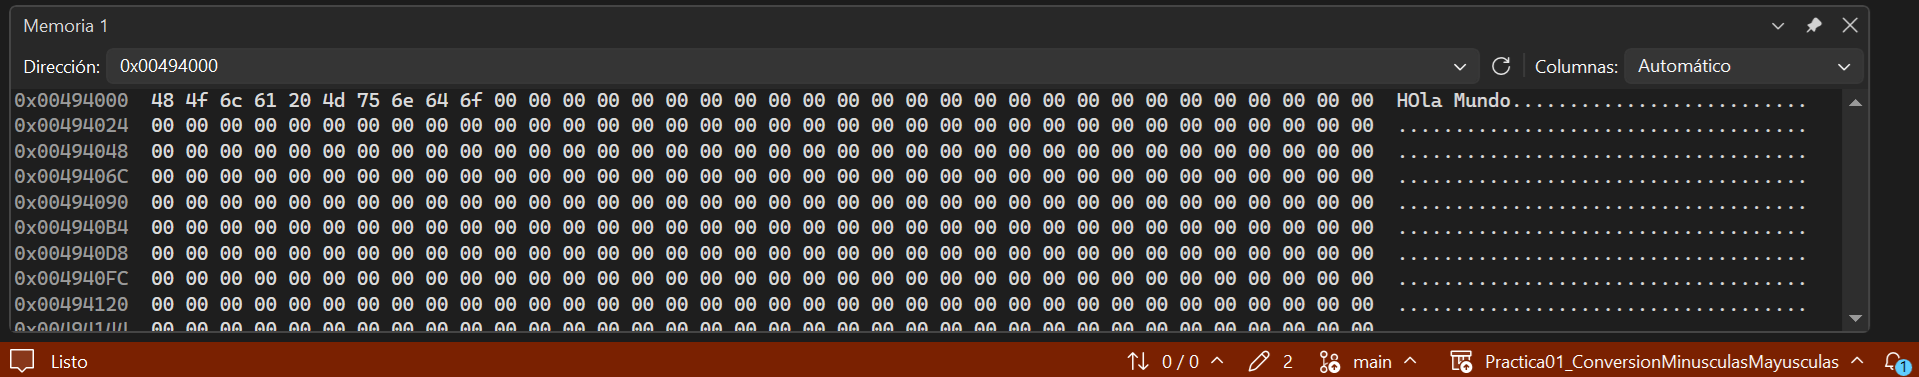
\includegraphics[width=1\textwidth]{memoria_01.png}
    \caption{Registros de memoria con "Hola Mundo"}
    \label{fig:etiqueta}
\end{figure}

\begin{verbatim}
Después de ejecutar: 48 4F 4C 41 20 4D 55 4E 44 4F 00
                     H  O  L  A     M  U  N  D  O  \0
\end{verbatim}

\begin{figure}[hbtp]
    \centering
    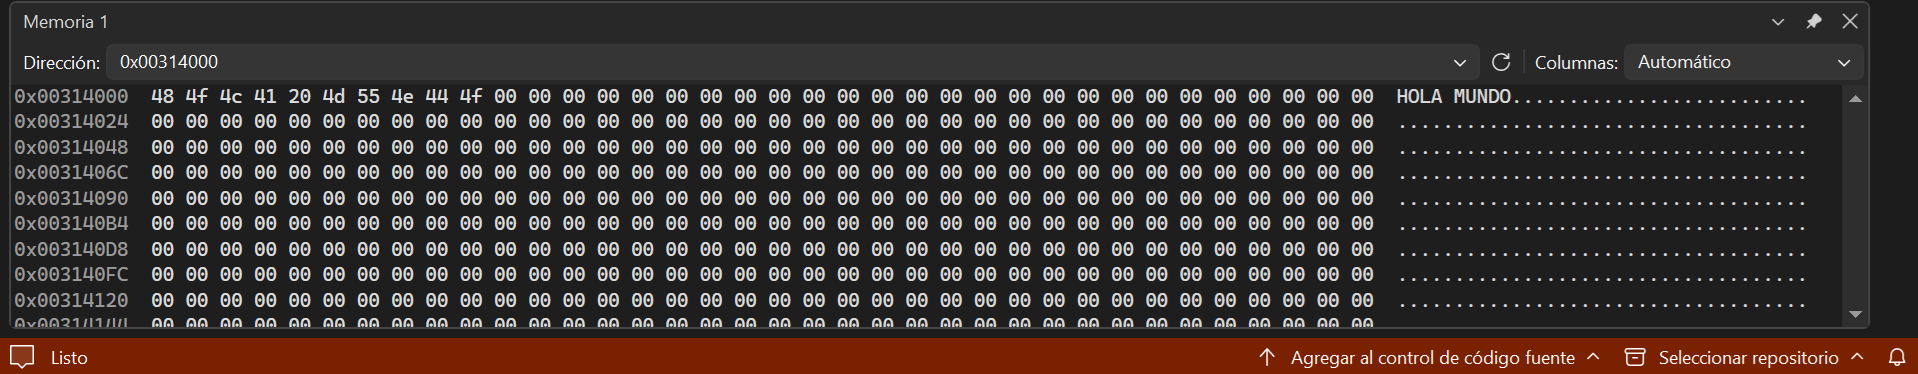
\includegraphics[width=1\textwidth]{memoria_02.png}
    \caption{Registros de memoria con "HOLA MUNDO"}
    \label{fig:etiqueta}
\end{figure}

% ============================================================
\section{Repositorio GitHub}

https://github.com/7mo-ArquitecturaComputadoras/Practica01\_ConversionMinusculasMayusculas

% ============================================================
\section{Conclusiones}

\begin{itemize}
    \item El programa demuestra que \textbf{trabajar con texto en ensamblador es trabajar con números}: las letras son valores enteros en la tabla ASCII, y su manipulación se reduce a operaciones aritméticas simples.
    \item La diferencia de 32 entre las mayúsculas y las minúsculas en la tabla ASCII no es accidental; fue un diseño deliberado que facilita exactamente este tipo de conversión con una sola resta.
    \item El uso de \textbf{registros como punteros} (\texttt{ESI}) es un patrón fundamental en ensamblador para recorrer estructuras de datos en memoria, equivalente a un índice de arreglo en lenguajes de alto nivel.
    \item El \textbf{filtro de rango} (verificar que el valor esté entre 97 y 122) es indispensable: sin él, el programa restaría 32 a espacios, números y mayúsculas, corrompiéndolos.
    \item Esta práctica evidencia lo que sucede ``detrás de escenas'' cuando un lenguaje como Python o Java convierte texto a mayúsculas con una función: al fondo, el procesador realiza exactamente esta misma secuencia de comparaciones y restas.
\end{itemize}

\end{document}
